\documentclass[10pt,journal,compsoc]{IEEEtran}
\usepackage{amsmath}
\hyphenation{op-tical net-works semi-conduc-tor}
\usepackage{graphicx}
\usepackage{soul} %for highlighting
\usepackage{listings} %for code syntax
\lstset{language=Lisp} %set to LISP!

\begin{document}
\begin{titlepage}
	\centering
	{\scshape Massachusetts Institute of Technology  \par}
	\vspace{3cm}
	{\scshape\LARGE 6.945: Large Scale Symbolic Systems\par}
	\vspace{1cm}
	{\scshape\Large Final Report \par}
	\vspace{1.5cm}
	{\huge\bfseries Debugging, Better\par}
	\vspace{2cm}
	{\Large\itshape Kenneth Friedman\par}
		{\Large\itshape Blake Elias \par}
			{\Large\itshape Jared Pochtar \par}
	\vspace{.25cm}
	\textit{{\small ksf@mit, eliasb@mit.edu, jpochtar@college.harvard.edu}}
	\vfill
    Professor Gerald Jay Sussman\par
	Manushaqe Muco

	\vfill

	{\large May 15, 2017\par}
\end{titlepage}

\twocolumn[
	\begin{abstract}
		To more easily write large scale, robust systems, it is necessary to improve our debugging tools and methods. In this project, we explore new methods of debugging Scheme. By implementing a fully working programming environment (also known as an integrated development environment, or IDE), we demonstrate major improvements to current debugging methods. The IDE contains three major components: a highlight to evaluate system, a way to manipulate values by dragging, and expression investigation.\\
		\\
		Here, we first explain the motivation beind our IDE. Then, we describe our environment and how it communicates with Scheme. Next, we describe the major debugging components in detail, and describe their implementation. Finally, we summerize our findings and describe future possibilities.
		
	\end{abstract}
	\centering\IEEEcompsocdiamondline\vspace{.5cm}]

	% The paper headers
	\markboth{6.945: Large Scale Symbolic Systems, MIT, Spring 2017}{}
		
		\section{Motivation}
		"Programs must be written for people to read, and only incidentally for machines to execute" -Abelson and Sussman, SCIP\\
		\\
		"Debugging is twice as hard as writing the code in the first place." -Brian W. Kernighan\\
        \\
        Kernighan wrote those words in 1978, and they are still true today. Our vision for this project is introduce a brand new Scheme programming environment that makes major improvemnts to debugging. While this is in a prototype state, we have a fully working implementation that can already help you better understand your code.
        \\
        To take steps towards our vision, we implemented a Scheme IDE with debugging tools built into the environment. We designed our environment with specific design goals in mind. We also have three major subsystems to our IDE. Here, we will describe our design goals and major subsystems in brief.
        
        \subsection{Design Goals}
        
        Our main goal is to demonstrate that new ideas and techniques in debugging can improve the overall programming experience. In terms of design goals, we followed the major guidelines of the project. Our "mix and match pieces" are the distinct debugging tools, which can be swapped and replaced without harm to the system. Our system is also robust, and incremental changes to the tools will only require incremental changes to the code. Each major system subsystem can be swapped for a different implementation. Finally, the project is well documented, and can be easily run and modified, without the need for dependencies.
        
        \subsection{Subsystems}
        Each subsystem in our IDE (which has the working name: \emph{Schemer}) is a debugging feature. We have three main debugging features.\\
        \\
        First, our system includes "Highlight to Preview". This introduces a new concept of a preview-execution. You can temporarily see the output of your code (by selecting a section of text), and then instantly "undo" the computation (by deselecting that text).\\
        \\
        Second, our system includes draggable manipulation. This alows you to easily see the output of a procedure over a range of numerical inputs. Simply hover over a numberical value, and "drag" by pressing and panning the pointer to the left (to decrease the value) or right (to increase the value). The function will automatically compute based on the new value.\\
        \\
        Third, Schemer contains a method to explore expressions, known as Expression Investigation. This allows a user to slowly drill down into a procedure, to understand it's "trace," without having to use breakpoints or mannual investigations. 
        
        \begin{figure}
            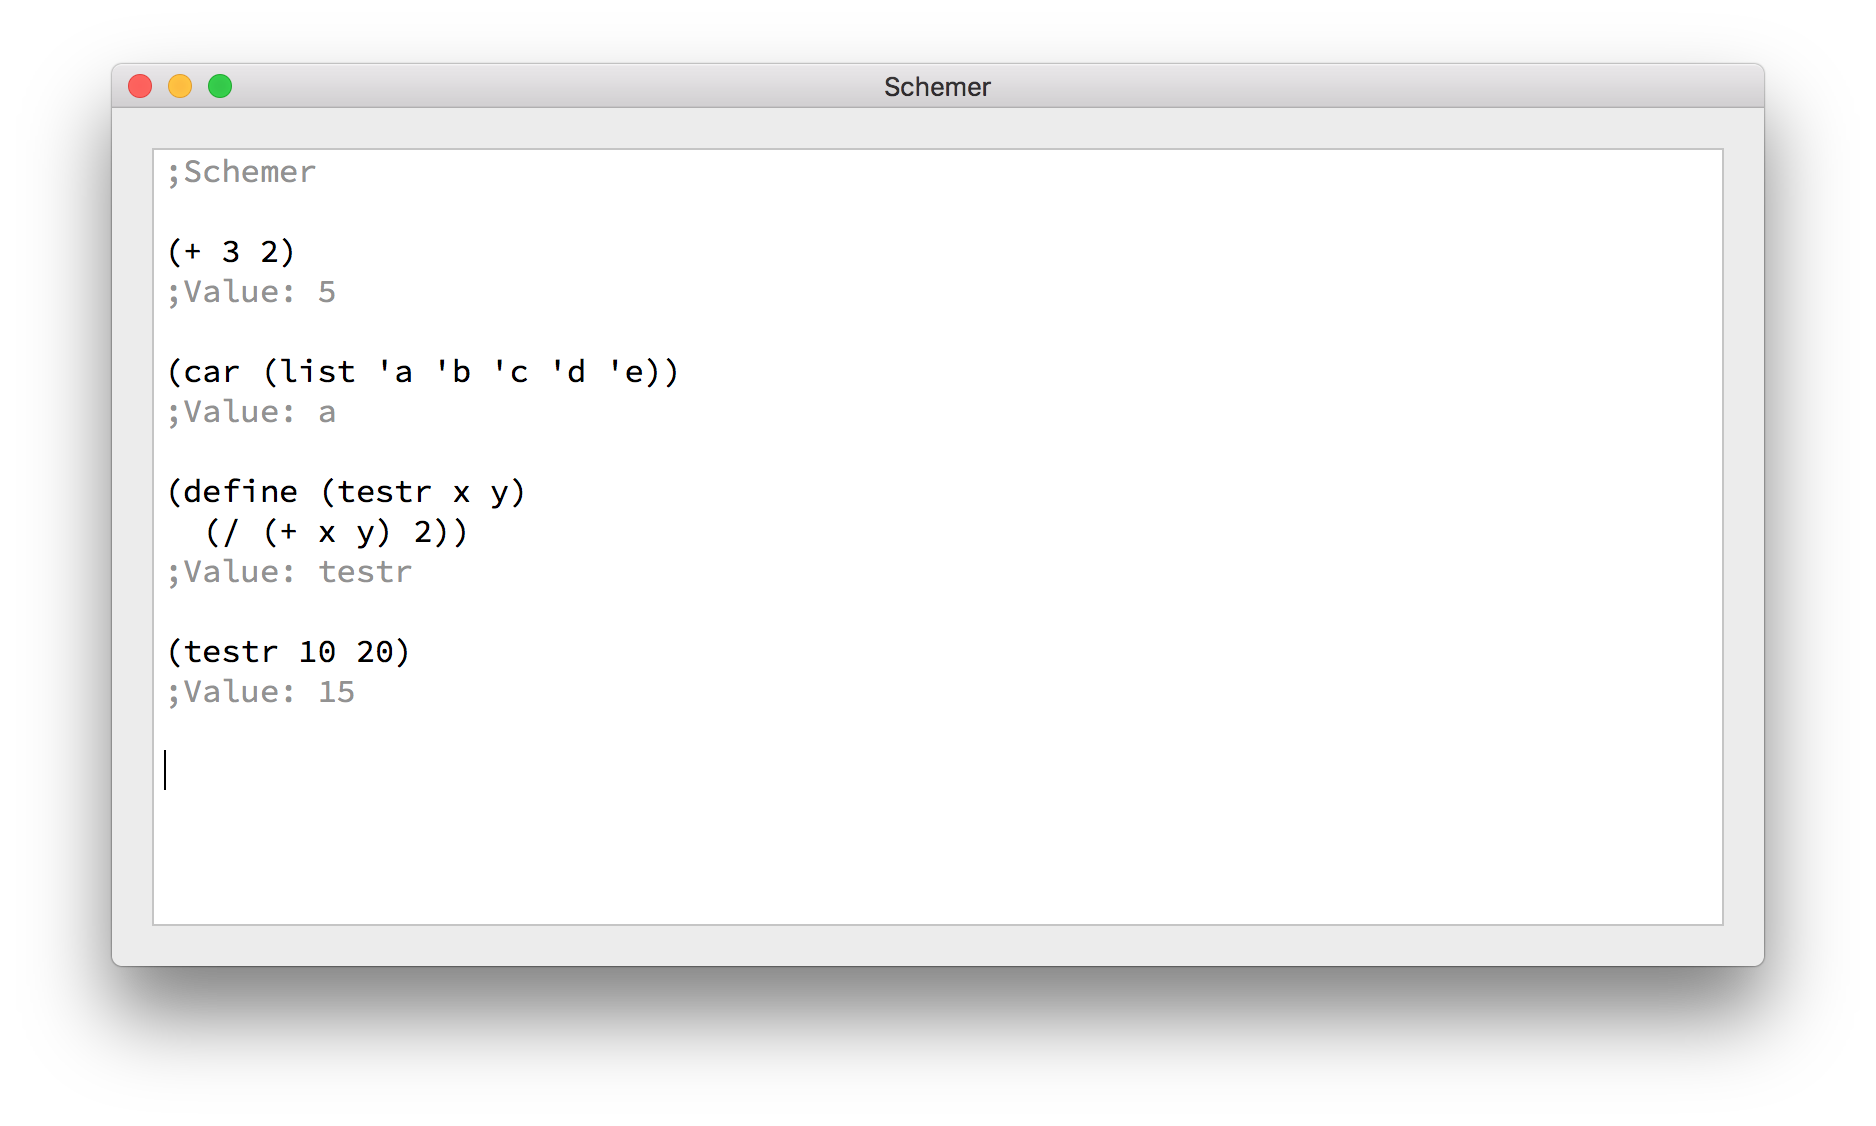
\includegraphics[width=\linewidth]{preview-1.png}
            \caption{A Screenshot of \emph{Schemer}, the working name for our debugging IDE. The graphical user interface handles the input and output of Scheme execution. Similar to using \emph{Emacs} with MIT-Scheme, it is not a REPL. The user is free to place their cursor at any point in the document and execute commands anywhere and in any order. Like building with mud, the user has the freedom!}
            \label{fig:overview}
        \end{figure}

		\section{Schemer, the IDE}
		The base level IDE (which is everything before the debugging tools) includes two major components, a "frontend" Mac app GUI, and a "backend" pipe to an MIT Scheme REPL process.\\
		\\
		The Mac app GUI gives the appearance of a straightforward text field. It takes input from the keyboard and watches for interactions (such as highlighting, cursor movement, and execution commands). It displays the input from the user and also sends the input to the the backend pipe. Finally, the frontend receives a stream of data from the backend pipe (which is the result of Scheme computation), and then displays the result to the user. The GUI also provides syntax highlighting: for example, comments are shown in a gray font while code is in black.\\
		\\
		The backend pipe is constantly listening to the frontend, waiting for data. Once data is received, it sends it to the Scheme process that it owns. This backend pipe operates on a seperate thread from the front end, so large computations do not slow the interaction of the frontend. Once the computation is complete, it sends the result back to the frontend to be displayed as text to the user.\\
		\\
		Both the Mac app GUI and the backend pipe are written in Swift 3. Swift is an open source language (more information, here: https://swift.org ). The Schemer IDE requires no dependencies to run other than the base level OS version: which is MacOS 10.10. It would be possible to port to other operating systems: the native graphic elements of the app are the only thing preventing it from running elsewhere.
		
		\section{Major Subsystems / Debugging Tools}
		
		Next, we explain the major subsystems to the IDE.
	    
	    \begin{figure}
            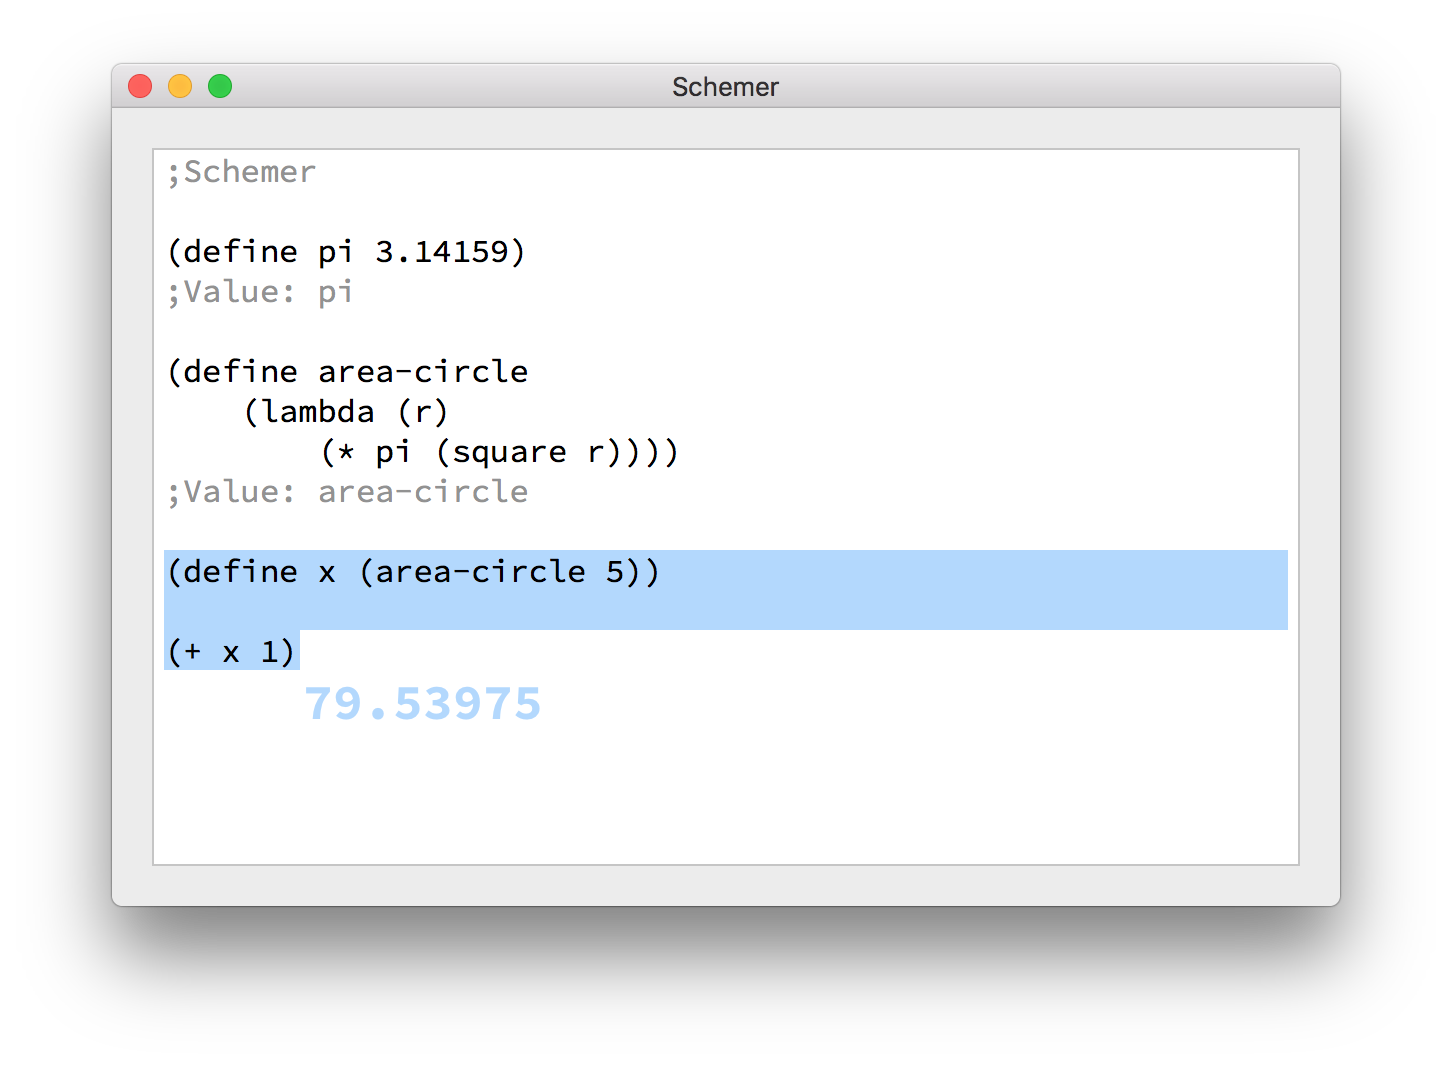
\includegraphics[width=\linewidth]{preview-2.png}
            \caption{The Highlight to Evaluate tool in \emph{Schemer}. Simply select the text you want to execute, and you will see a preview of the value if you were to execute the command. However, the command does not really execute (from the user's perspective). Once they let go, if they were to just run the \lstinline{(+ x 1)} command, there would be an error: because \lstinline{x} is unbound.}
            \label{fig:overview}
        \end{figure}
	    
	    
	    \subsection{Highlight to Evaluate}
	    
	    This features introduces a new concept to Scheme programming: a “preview execution”. A Preview Execution is temporary: It allows a user to see the result of their code, and then immediately undo the fact that the code was executed.\\
	    \\
        In our debugger, you can simply highlight a section of code, and it will execute a preview. It will show you the result of the execution while the text remains highlighted. However when you deselect the text, any mutated state is automatically removed: as if the execution never took place.\\
        \\
        For example, consider the following:
        \begin{lstlisting}[frame=single]
(define x 5)
;Value: x

(define x 10)
(+ x 1)

(+ x 3)
        \end{lstlisting}
        
        If the programmer selects the highlighted the 3rd and 4th lines of text above, they will see the value \lstinline{11}. However, if they then highlight the final line, \lstinline{(+ x 3)}, they will see the value \lstinline{8}, as the environment gets reset to the old value of \lstinline{x}, which was \lstinline{5}.\\
        \\
        The behind-the-scenes implementation of this involves using Scheme environments, duplicating the environment and modifying its state, and then removing the new environment when the Preview Execution is complete.

        \subsection{Draggable Manipulation}
        
        This feature allows the programmer to inspect the execution of their program. A programmer may wish to see exactly how an expression evolves into its final value, in a step-by-step manner. By highlighting an expression and clicking “expand”, the programmer can see the expression generated by substituting a function’s arguments into the function body. For example with \lstinline{(factorial 4)}, highlighting the expression will show \lstinline{24}, but clicking the “expand” button will substitute \lstinline{4} into the function body of “factorial”, showing \lstinline{(* 4 (fact 3))}. From here, the programmer can further expand \lstinline{(fact 3)} into \lstinline{(* 3 (fact 2))}, and so forth. 

The programmer can also replace a complex expression with its value by clicking “replace by value”. For example, suppose the expression in question is \lstinline{(* 4 (* 3 (fact 2)))}. The programmer may highlight \lstinline{(* 3 (fact 2))}, at which point they will see its value as \lstinline{6} in a preview execution). But then they can click “replace by value” to permanently substitute in the \lstinline{6}, making the overall expression read as \lstinline{(* 4 6)}. At this point the programmer can easily see why the final value came out to be 24. 

        \subsection{Expression Investigation}
        
        Any numerical literal value in Schemer becomes draggable when the programmer hovers on that value in the source code, indicated by a double-arrowed cursor. If the programmer subsequently clicks and drags left or right, the literal value changes and the output (displayed on the right-hand-side) changes along with it. Dragging left makes the value decrease, and dragging right makes it increase, preserving the original type (integer or floating point are the types supported currently). 

There is support for future extensions of this functionality to other types as well. For example, strings or lists could also be made draggable. The programmer would just have to define what it means to “increment” and “decrement” those types: add or remove one character from the string, add repeated elements to the list, etc. 
		
		\section{Contributions}
		Here, we have demostrated a prototype, yet working, IDE for Scheme that includes debugging tools to enhance the programming experience. We introduced three major subcomponents and explained their features. In the future, debugging will not be as hard as it was for Kernighan at Bell Labs.
		
		\section{Acknowledgments}
		The authors would like to thank Professor Sussman and Manushaqe Muco for the adventures.
		
\end{document}























































\end{document}